\label{chap:jueces}

En esta sección se resolverán 2 problemas relacionados con \textit{string matching} usando el
algoritmo KMP y la función de error de la que se habló en el capítulo 4. Se resolverán los
problemas usando C++ y Haskell y se compararán ambas versiones.

Es un estándar que las especifiaciones del problema estén en inglés.

%% TODO: Explicar los constraints

\section{SPOJ}
SPOJ (Sphere Online Judge)
% https://wiki.haskell.org/SPOJ
% Tomar algo del competitive aquí

\section{Problemas}

% TODO: poner aquí la motivación.

\subsection{Encontrar el factor de repetición de una cadena}
Recordemos en el \hyperlink{repetition_factor}{capítulo 3 el problema 32.1}, es aquí cuando lo
bonito de la programación competitiva y resolver ejercicios teóricamente se juntan. Ése problema
es lo mismo a resolver el siguiente, y aún mejor, en un juez en línea que puede ``probar'' la
implementación considerando ciertas restricciones.

La especificación del problema dice lo siguiente: 

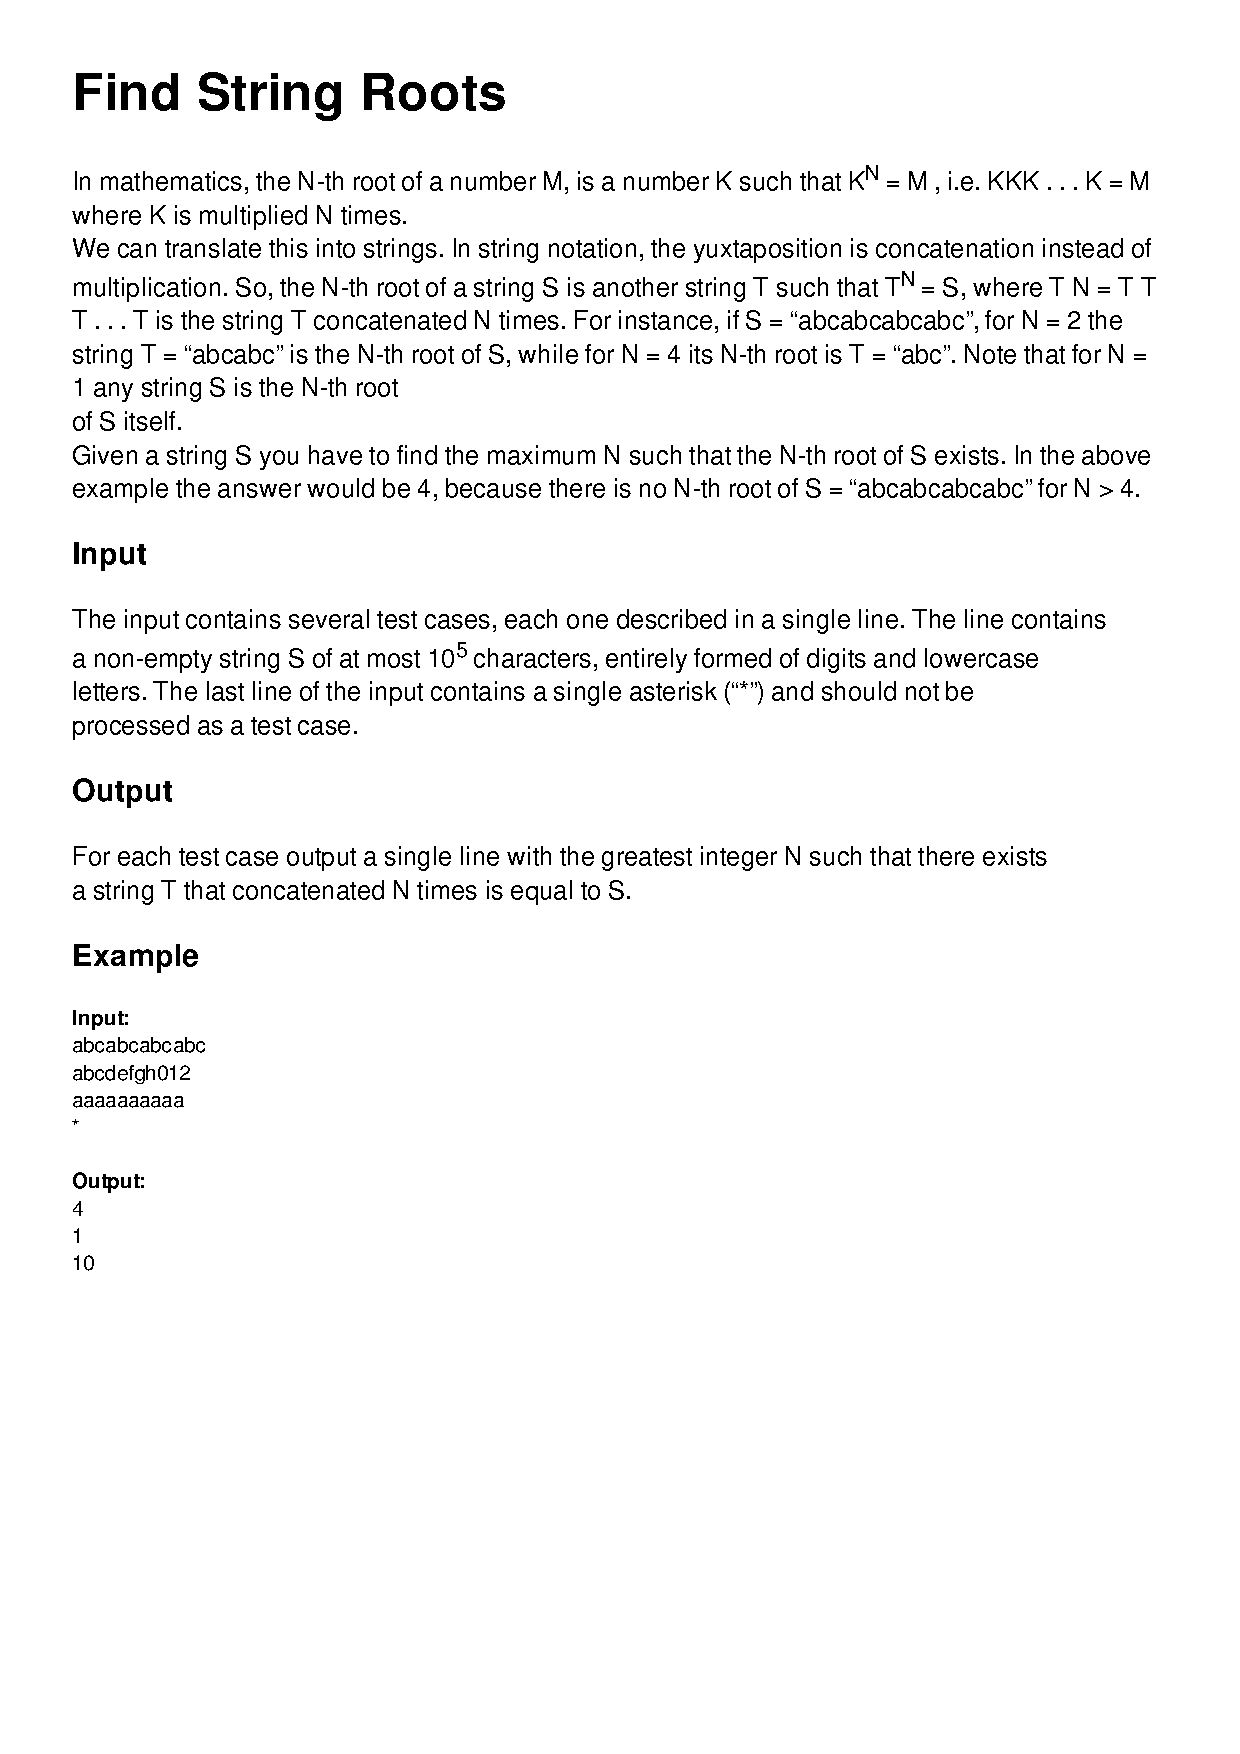
\includepdf[pages=-]{problemas/pdf/FINDSR.pdf}

\subsubsection{Análisis}
Como se había dicho previamente, ya se había atacado este problema así que se omitirá el análisis
y la complejidad.

\subsubsection{Entrada}
Una \textit{heurística} a seguir es que siempre que diga: \textit{``the input contains several test
cases, each line described in a single line''} es leer hasta el final de archivo (End Of File) cada
línea. Seguido de esto, dice que cada línea una cadena no vacía de a lo más $10^5$
caracteres\footnote{Hay lenguajes programación que no tienen implementadas cadenas, y que se debe
saber de antemano el tamaño, para así tener un arreglo de $n$ caracteres. Es aquí cuando es
importante saber el tamaño máximo de la entrada.} formada solamente de dígitos y letras en
minúsculas\footnote{También es sumamente importante saber si las cadenas del lenguaje que se usará
como son represntadas ya que podrían estar en ASCII o Unicode.}.
Finalmente dice que la última entrada contiene un solo asterisco \texttt{*} y que no debe ser
procesado como un caso más.

\subsubsection{Salida}
Para cada caso prueba \textit{(input)} se debe imprimir en la salida estándar una sola línea con un
número $n$ siendo ésta la raíz de la cadena, es decir, el número de veces que está concatenada la
cadena consigo misma.

\subsubsection{Ejemplos}
\begin{itemize}
\item Consideremos la entrada $x =$ \texttt{abcabcabcabc} y sobre ésta se construye la función
de error, 
\begin{table}[h]
\centering
\begin{tabular}{c|c|c|c|c|c|c|c|c|c|c|c|c|}
\cline{2-13}
$i$      & 1          & 2          & 3          & 4          & 5          & 6          & 7          & 8          & 9          & 10         & 11         & 12         \\ \hline
$P[i]$   & \texttt{a} & \texttt{b} & \texttt{c} & \texttt{a} & \texttt{b} & \texttt{c} & \texttt{a} & \texttt{b} & \texttt{c} & \texttt{a} & \texttt{b} & \texttt{c} \\ \hline
$\pi[i]$ & 0          & 0          & 0          & 1          & 2          & 3          & 4          & 5          & 6          & 7          & 8          & 9          \\ \cline{2-13} 
\end{tabular}
\end{table}

Siendo $\vert x \vert = 12$ y el último elemento de la función de error es $\pi[m] = 9$ y sea
$r = 12 - 9 = 3$. Se conluye que la raíz de la cadena es de longitud \textbf{3} y su factor de
repetición es $\rho(x) = \frac{12}{3} =$ \textbf{4}. Concluyendo así que
\texttt{(abc)}$^4 = $ \texttt{abcabcabcabc}.

\item Consideremos la entrada $x =$ \texttt{acbdefgh012} y sobre ésta se construye la función
de error, 
\begin{table}[h]
\centering
\begin{tabular}{c|c|c|c|c|c|c|c|c|c|c|c|}
\cline{2-12}
$i$      & 1          & 2          & 3          & 4          & 5          & 6          & 7          & 8          & 9          & 10         & 11         \\ \hline
$P[i]$   & \texttt{a} & \texttt{b} & \texttt{c} & \texttt{d} & \texttt{e} & \texttt{f} & \texttt{g} & \texttt{h} & \texttt{0} & \texttt{1} & \texttt{2} \\ \hline
$\pi[i]$ & 0          & 0          & 0          & 0          & 0          & 0          & 0          & 0          & 0          & 0          & 0          \\ \cline{2-12} 
\end{tabular}
\end{table}

Siendo $\vert x \vert = 11$ y el último elemento de la función de error es $\pi[m] = 0$ y sea
$r = 11 - 0 = 11$. Teniendo que su factor de repetición es $\rho(x) = $ \textbf{1}. Concluyendo
así que\texttt{(acbdefgh012)}$^1 = $ \texttt{acbdefgh012}.

\item Consideremos la entrada $x =$ \texttt{aaaaaaaaaa} y sobre ésta se construye la función
de error, 
\begin{table}[h]
\centering
\begin{tabular}{c|c|c|c|c|c|c|c|c|c|c|}
\cline{2-11}
$i$      & 1          & 2          & 3          & 4          & 5          & 6          & 7          & 8          & 9          & 10         \\ \hline
$P[i]$   & \texttt{a} & \texttt{a} & \texttt{a} & \texttt{a} & \texttt{a} & \texttt{a} & \texttt{a} & \texttt{a} & \texttt{a} & \texttt{a} \\ \hline
$\pi[i]$ & 0          & 1          & 2          & 3          & 4          & 5          & 6          & 7          & 8          & 9          \\ \cline{2-11} 
\end{tabular}
\end{table}

Siendo $\vert x \vert = 10$ y el último elemento de la función de error es $\pi[m] = 9$ y sea
$r = 10 - 9 = 1$. Se conluye que la raíz de la cadena es de longitud \textbf{1} y su factor de
repetición es $\rho(x) = \frac{10}{1} =$ \textbf{1}. Concluyendo así que
\texttt{(a)}$^{10} = $ \texttt{aaaaaaaaaa}.
\end{itemize}
\newpage

\subsubsection{Implementación en C++}
\inputminted[linenos, frame=lines, fontsize=\footnotesize]{cpp}{problemas/cpp/FINDSR.cpp}

\begin{itemize}
\item En la línea \texttt{1} se agrega la cabecera \texttt{iostream} que define la entrada y salida
estándar. En la línea \texttt{2} se agrega la cabecera \texttt{vector} que son contenedores de
arreglos dinámicos.

\item De línea \texttt{6} a \texttt{19} es la implementación de la función de error.

\item En la línea \texttt{23} es la parte importante sobre leer la entrada; se leerá hasta EOF y si
la cadean leída es diferente de \texttt{*}.

\item En la línea \texttt{24} se crea un vector con la función de error con el patrón \texttt{s}, y
en la línea \texttt{28} se obtiene la posible longitud de la $k$-ésima raíz del patrón.

\item Y de la línea \texttt{30} a \texttt{33} es cuando se hace la validación previamente analizada.
\end{itemize}

\subsubsection{Implementación en Haskell}
\inputminted[linenos, frame=lines]{haskell}{problemas/haskell/FINDSR.hs}

\begin{itemize}
\item En la línea \texttt{1} del módulo \hsCode{Data.Array} importamos solamente el tipo
\hsCode{Array} sin ninguno de sus constructores, la función \hsCode{bounds :: Array i e -> (i, i)}
que devuelve los límites del arreglo en cual fue construido,\\
\hsCode{listArray :: Ix i => (i, i) -> [e] -> Array i e} que construye un arreglo donde el primer
argumentos son los límites inferiores y superiores, y una lista de valores devolviendo valores
con un orden indexado,\\
\hsCode{(!) :: Ix i => Array i e -> i -> e}  regresa el valor de un índice dado en el arreglo.

\item Analicemos parte por partes las líneas \texttt{3, 4}. recordemos la función \\
\hsCode{interact :: (String -> String) -> IO ()}, la función \hsCode{interact} toma una función de
tipo \hsCode{(String -> String)} como argumento. La \textit{entrada} entera de la entrada estándar
es pasada a ésa función como argumento, y la cadena resultante es la \textit{salida} de la
salida estándar.

Acto seguido, se tiene la función \texttt{\$} que es un operador infijo con asociatividad izquierda,
esto para tener mejor legibilidad cuando se tienen argumentos largos.

Dado que se procesará linea por línea de la entrada, es bastante común tratar el flujo de la
entrada como una lista de líneas, así que para hacer eso se divirá todo la cadena de entrada en
líneas. Consideremos las funciones\\ \hsCode{lines :: String -> [String]} y
\hsCode{unlines :: [String] -> String}, donde\\ \hsCode{lines} divide la cadena en una lista de
cadenas cuando se encuentra un caracter de salto de línea, \hsCode{unlines} es la operación inversa
de \hsCode{lines}, une líneas y después añade un caracter de salto de línea a cada cadena.

Pongamos total atención a la siguiente composición de funciones\\
\hsCode{unlines . map parse . takeWhile (/= "*") . lines}.\\
La función \hsCode{map parse} será la responsable de que la cadena en turno la tranformará a la
respuesta del problema.

La función \hsCode{takeWhile :: (a -> Bool) -> [a] -> [a]}, aplicado a un predicado \hsCode{p} y
una lista \texttt{xs}, regresa el prefijo más largo (que posiblemente puede ser vacío) de
\texttt{xs} de los elemetos que satisfacen \hsCode{p}.
Entonces \hsCode{takeWhile (/= "*")} significa que se seguirá procesanso hasta que la cadena leída
sea diferente de \texttt{*}.

El patrón \hsCode{unlines . f . lines} es un patrón bastamte común donde \hsCode{f} puede ser una
función o composición de funciones donde \hsCode{f :: [String] -> [String]}.

\item De la línea \texttt{6, 7} la función \hsCode{parse} será la responsable de tomar la cadena en
turno, tomar el resultado de \hsCode{process} y convertirlo al tipo \hsCode{String}.

En el punto siguiente se hablará sobre la función \hsCode{process :: String -> Int}, pero básicamente es
la que ``hará el algoritmo'', lo importame aquí es el tipo \hsCode{Int}, y es por eso que se hizo
la función \hsCode{parse :: String -> String}.

\item De igual manera de las líneas \texttt{8} a \texttt{16} en la expresión \hsCode{let ... in ...}
en la línea \texttt{10} se calcula la función de error de la cadena de entrada, en la \texttt{11}
se obtienen los límites del arreglo siendo la segunda entrada tamaño del arreglo, y en la línea
\texttt{12} se obtiene el último elemento del arreglo y después su índice. En la línea \texttt{13}
se obtiene la posible longitud de la $k$-ésima raíz del patrón. Finalmente de la línea \texttt{14}
a \texttt{16} es cuando se hace la validación previamente analizada.

\item De la línea \texttt{19} a \texttt{29} es la implementación de función de error.
\end{itemize}

\subsubsection{Resultado del juez}
\begin{figure}[H]
\centering
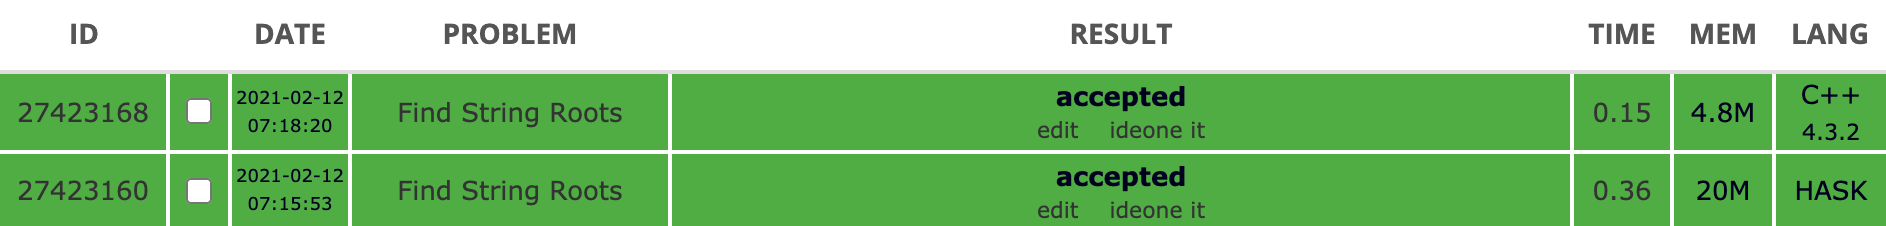
\includegraphics[width=\textwidth]{spoj/FINDSR-accepted-cpp-haskell}
\caption{El código fue aceptado por el juez en Haskell y C++}
\end{figure}

\newpage


\subsection{Ver si una cadena es una rotación cíclica de otra}

\subsubsection{Análisis}
De igual manera, el en \hyperlink{cyclic_rotation}{capítulo 3 el problema 32.4-7} se había hecho el
análisis del problema, y como este problema es resovler exactamente lo mismo se omitirá el análisis
y su complejidad.

\subsubsection{Entrada}
Este tipo de entrada es la más común que se verá en la programación competitiva; ya que la primera
línea será un entero con el número de casos a resolver, después caso consistirá de dos líneas.

Igual que el problema anterior (e igual que en la mayoría de los problemas de este índole) la
entrada será sobre un alfabeto de \texttt{[a-z]} entonces serán representados en ASCII.

\subsubsection{Salida}
Solo se deberá mostrar en la salida estándar \texttt{Si} o \texttt{No} dependiendo si es una
rotación cíclica.

\subsubsection{Ejemplos}
Dado que ambas cadenas son de la misma longitud se hará lo siguiente, $s = qq$ donde $s$ será el
texto y $p$ el patrón. Entonces con el algoritmo dee Knuth-Morris-Pratt se buscará $p$ en $s$.

\begin{itemize}
\item \texttt{abc} es una rotación cíclica de \texttt{cab} porque \texttt{cab} $\mapsto$
\texttt{abc}. Se muestra en la siguiente tabla de manera gráfica la idea.
\begin{table}[h]
\centering
\begin{tabular}{|c|c|c|c|c|c|}
\hline
\texttt{c}                   &  \cellcolor{green}\texttt{a} &  \cellcolor{green}\texttt{b} &
\cellcolor{green} \texttt{c} &  \texttt{a}                  & \texttt{b}                   \\\hline
\end{tabular}
\end{table}

\item Claramente \texttt{abab} no es rotación cíclica de \texttt{aabb}.
\begin{table}[h]
\centering
\begin{tabular}{|c|c|c|c|c|c|c|c|}
\hline
\texttt{a} & \texttt{b} & \texttt{a} &\texttt{b} & \texttt{a} & \texttt{b} & \texttt{a} & \texttt{b} \\\hline
\end{tabular}
\end{table}
\end{itemize}

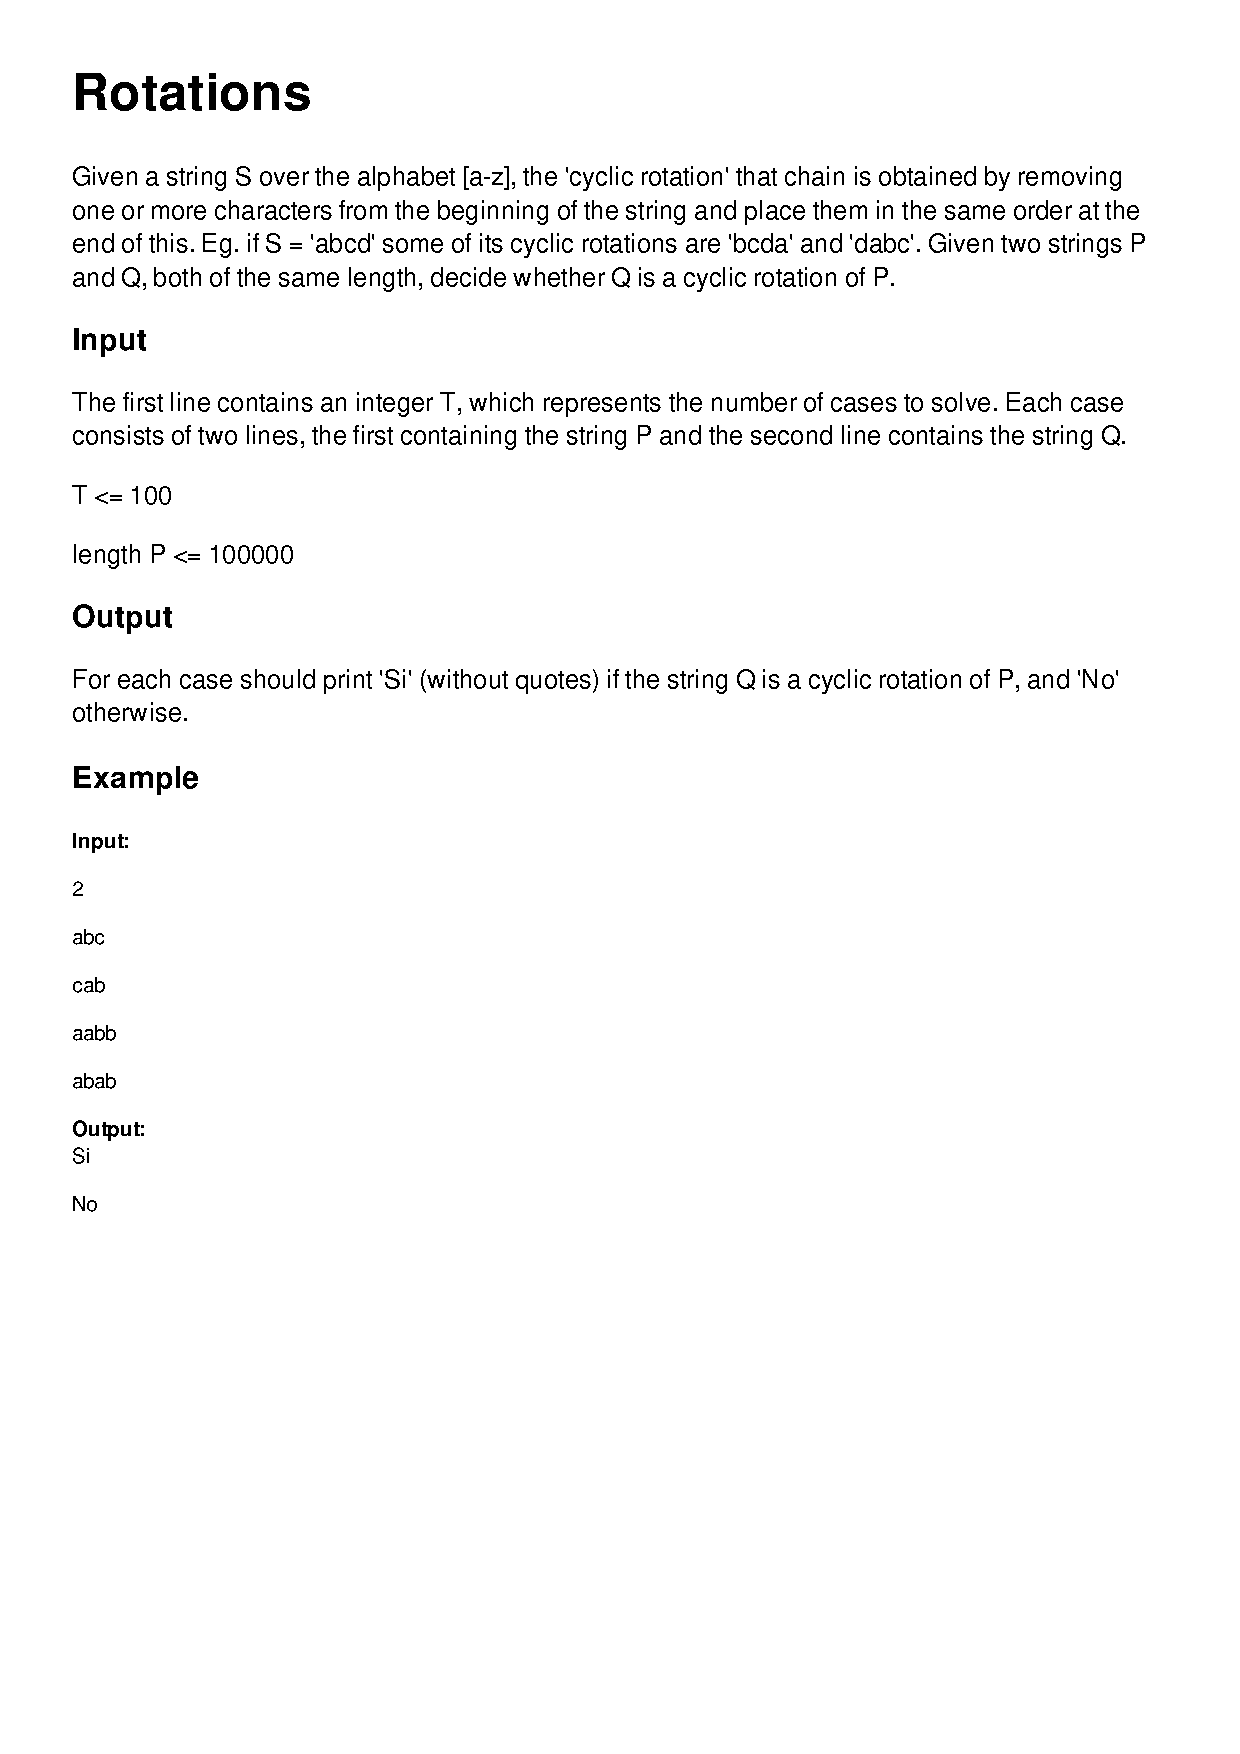
\includepdf[pages=-]{problemas/pdf/EC_WORLD.pdf}

\subsubsection{Implementación en C++}
\inputminted[linenos, frame=lines, fontsize=\footnotesize]{cpp}{problemas/cpp/EC_WORLD.cpp}
\begin{itemize}
\item De línea \texttt{6} a \texttt{19} es la implementación de la función de error.

\item De línea \texttt{21} a \texttt{38} es la implementación del algoritmo Knuth-Morris-Pratt.

\item En línea \texttt{43} se lee el número de casos, y en la \texttt{44} se itera \texttt{t} hasta
que sea 0 y como cualquier valor no cero en \texttt{while} lo toma como falso para la iteración.

\item De la línea \texttt{47} a \texttt{52} es cuando hace la validación dicha en el análisis.

\end{itemize}

\newpage

\subsubsection{Implementación en Haskell}
\inputminted[linenos, frame=lines]{haskell}{problemas/haskell/EC_WORLD.hs}

Muchas veces algunos jueces no aceptan cierto lenguaje, y en este caso el que diseñó el problema y
lo subió en SPOJ, no puso a Haskell para este problema. Pero aún así se hará.

Dado que el tipo de entrada, que es por casos es diferente al problema anterior, la naturaleza de
la entrada y salida será diferente.

\begin{itemize}
\item En la línea \texttt{1} del módulo \hsCode{Control.Monad} se importa la función\\
\hsCode{replicateM :: Applicative m => Int -> m a -> m [a]}, donde\\ \hsCode{replicateM n act}
lleva a cabo una acción $n$ veces, juntando los resultados.

\item De la línea \texttt{4} a \texttt{8} empieza el bloque \hsCode{do} utilizado para las
operaciones de entrada y salida como secuencia.

En la línea \texttt{5} lee una línea, que es el número de casos de la entrada estándar y eso es
transformado con \hsCode{fmap :: (a -> b) -> f a -> f b} a un entero con la función
\hsCode{read :: Read a => String -> a}. Se ocupa el sinónimo infijo \texttt{<\$>} de \hsCode{fmap}.

En la línea \texttt{6} es cuando se lee la entrada de cada caso, primero \hsCode{replicateM t}
ejecuta la acción \hsCode{replicateM 2 getLine} $t$ veces, donde cada una lee de la entrada
estándar 2 veces.

En la línea \texttt{7} como la expresión \hsCode{let} está en el bloque \hsCode{do} se omite el
\hsCode{in} después. Dado que \hsCode{inputs} tiene ligado los valores de la entrada, cada caso que
consiste de una lista de dos elementos es transformado con \texttt{<\$>} por la función
\hsCode{process} que hace el ``algoritmo'' descrito en el análisis.

En la línea \texttt{8} en la función\\
\hsCode{sequence_ :: (Foldable t, Monad m) => t (m a) -> m ()}, que evalúa cada acción monádica de
la estructura plegable de iquierda a derecha e ignora sus resultados, los hacemos porque serán
puras acciones \hsCode{IO ()}, \hsCode{sequence_} recibe como argumento acciones monádicas donde
cada \texttt{answer} se imprime en la salida estándar con \hsCode{putStrLn :: String -> IO ()}. 

\item De la línea \texttt{10} a \texttt{16} es see crea la función
\hsCode{process :: [String] -> String}, donde por medio de caza de patrones se trabaja con una
lista de dos elementos, acto seguido en la expresión \hsCode{let ... in ..} se busca la ocurrencia
del patrón \texttt{p} en \texttt{s} y al final con la función
\hsCode{null :: Foldable t => t a -> Bool} se verifica si la lista es vacía.  

\item De la línea \texttt{19} a \texttt{24} es la implementación del algoritmo Knuth-Morris-Pratt
funcionalmente.
\end{itemize}

\subsubsection{Resultado del juez}
\begin{figure}[H]
\centering
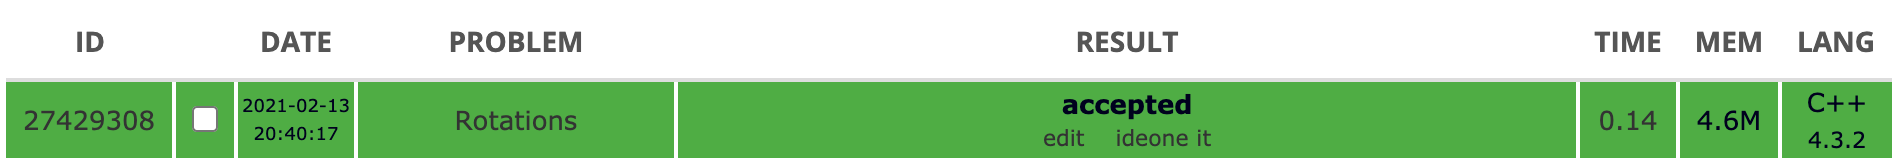
\includegraphics[width=\textwidth]{spoj/EC_WORLD-accepted-cpp}
\caption{El código fue aceptado por el juez en C++}
\end{figure}

\newpage


\subsection{Extender una cadena a un palíndromo}

\subsubsection{Análisis}
En este problema lo \textit{realmente importante} empieza en el tercer párrafo, que resumiendo es:

\begin{tcolorbox}
Dada una cadena, producir el palíndromo\footnote{Un palíndromo es una palabra o frase que se lee
igual en un sentido que en otro. Por ejemplo: arenera, oso, radar, sometemos, etc.} más corto que
puede ser formado agregando cero o más caracteres al final de la cadena.
\end{tcolorbox}

Una forma ingenua de resolver este problema es simplemente concatenando la cadena original $s$
con su reversa $s^R$, i.e., $t = ss^R$ donde $t$ ya es un palíndromo, y a pesar de que resuelve el
problema no se asegura que sea el palíndromo más corto.

Para mostrarlo tomemos una cadena arbitraria $s = $ \texttt{recono} y $s^R =$ \texttt{onocer}
quedando $t = $ \texttt{reconoonocer} y $t$ es un palíndromo pero hay un palíndromo más corto
$t' = $ \texttt{reconocer}. Esto fue concatenando \texttt{cer} a \texttt{recono}. 
Por lo tanto debe de haber una forma mejor de atacar el problema.

Consideremos la función de error utilizada en KMP, como por hipótesis del problema la cadena solo
consiste de letras mayúsculas y minúsculas, se puede usar un tipo de ``separador'' al procesar lo
siguiente; sea $r = s^R$\texttt{\$}$s$ donde $r$ es la concatenación de la reveresa de la cadena de
entrada concatenada con el símbolo \texttt{\$} como separador, y la cadena original.

Entonces se procesará $r$ con la función de error, y ésta indicará el prefijo más largo de $s^R$
que es sufijo de $s$, denominemos a tal la subcadena como $s'$ tal que $s' \sqsubset s^R$ y
$s' \sqsupset s$, esto para saber de antemano la subcadena que se traslapa en $s$ y $s^R$. Para
obtener $s'$ tomemos $n = \vert t \vert$ y $\pi$ la función de error donde $\pi[n] = k$ es la 
longitud de $s'$. Para finalmente tener el palíndromo más pequeño se toma la cadena original $s$
concatenada con $u = s^R[k \ldots]$ donde $u$ es la subcadena de $s^R$ desde $k$.

La complejidad del algoritmo es $\Theta(m)$ donde $m$ es el tamaño de la cadena de entrada tanto
en espacio y tiempo, esto es por construir la función de error y obtener la reversa de una cadena.

\subsubsection{Entrada}
Al igual que el primero problema, la entrada será leída línea por línea hasta EOF yla
entrada será sobre un alfabeto de \texttt{[a-z]|[A-Z]} entonces serán representados en ASCII.

\subsubsection{Salida}
Una sola línea que se imprime en la salida estándar con el palíndromo de más corto.

\subsubsection{Ejemplos}
\begin{itemize}
\item Sea $s = $ \texttt{aaaa}, $s^R =$ \texttt{aaaa} y finalmente
$r = s^R$\texttt{\$}$s =$ \texttt{aaaa\$aaaa} y se construye la función de error con $r$ quedando,

\begin{table}[h]
\centering
\begin{tabular}{c|c|c|c|c|c|c|c|c|c|}
\cline{2-10}
$i$      & 1          & 2          & 3          & 4          & 5           & 6          & 7          & 8          & 9          \\ \hline
$P[i]$   & \texttt{a} & \texttt{a} & \texttt{a} & \texttt{a} & \texttt{\$} & \texttt{a} & \texttt{a} & \texttt{a} & \texttt{a} \\ \hline
$\pi[i]$ & 0          & 1          & 2          & 3          & 0           & 1          & 2          & 3          & 4          \\ \cline{2-10} 
\end{tabular}
\end{table}
Para obtener $s'$ tomemos $n = \vert r \vert = 9$ y en $\pi[9] = 4$ donde $\vert s' \vert = 4$.\\
Siendo el palíndromo más corto como
$u = s \cdot s^R[4 \ldots] =$ \texttt{aaaa}$\cdot \varepsilon$ = \texttt{aaaa}.

\item Sea $s = $ \texttt{abba}, $s^R =$ \texttt{abba} y finalmente
$r = s^R$\texttt{\$}$s =$ \texttt{abba\$abba} y se construye la función de error con $r$ quedando,

\begin{table}[h]
\centering
\begin{tabular}{c|c|c|c|c|c|c|c|c|c|}
\cline{2-10}
$i$      & 1          & 2          & 3          & 4          & 5           & 6          & 7          & 8          & 9          \\ \hline
$P[i]$   & \texttt{a} & \texttt{b} & \texttt{b} & \texttt{a} & \texttt{\$} & \texttt{a} & \texttt{b} & \texttt{b} & \texttt{a} \\ \hline
$\pi[i]$ & 0          & 0          & 0          & 1          & 0           & 1          & 2          & 3          & 4          \\ \cline{2-10} 
\end{tabular}
\end{table}
Para obtener $s'$ tomemos $n = \vert r \vert = 9$ y en $\pi[9] = 4$ donde $\vert s' \vert = 4$.\\
Siendo el palíndromo más corto como
$u = s \cdot s^R[4 \ldots] =$ \texttt{abba}$\cdot \varepsilon$ = \texttt{abba}.

\item Sea $s = $ \texttt{amanaplanacanal}, $s^R =$ \texttt{lanacanalpanama} y finalmente\\
$r = s^R$\texttt{\$}$s =$ \texttt{lanacanalpanama\$amanaplanacanal} y se construye la función de
error con $r$ quedando,

\begin{table}[h]
\centering
\begin{tabular}{c|c|c|c|c|c|c|c|c|c|c|c|c|c|c|c|c|}
\cline{2-17}
$i$      & 1          & 2          & 3          & 4          & 5          & 6          & 7          & 8          & 9          & 10         & 11         & 12         & 13         & 14         & 15         & 16          \\ \hline
$P[i]$   & \texttt{l} & \texttt{a} & \texttt{n} & \texttt{a} & \texttt{c} & \texttt{a} & \texttt{n} & \texttt{a} & \texttt{l} & \texttt{p} & \texttt{a} & \texttt{n} & \texttt{a} & \texttt{m} & \texttt{a} & \texttt{\$} \\ \hline
$\pi[i]$ & 0          & 0          & 0          & 0          & 0          & 0          & 0          & 0          & 1          & 0          & 0          & 0          & 0          & 0          & 0          & 0           \\ \cline{2-17} 
\end{tabular}
\end{table}

\begin{table}[H]
\centering
\begin{tabular}{c|c|c|c|c|c|c|c|c|c|c|c|c|c|c|c|}
\cline{2-16}
$i$      & 17         & 18         & 19         & 20         & 21         & 22         & 23         & 24         & 25         & 26        & 27          & 28         & 29         & 30         & 31          \\ \hline
$P[i]$   & \texttt{a} & \texttt{m} & \texttt{a} & \texttt{n} & \texttt{a} & \texttt{p} & \texttt{l} & \texttt{a} & \texttt{n} & \texttt{a} & \texttt{c} & \texttt{a} & \texttt{n} & \texttt{a} & \texttt{l}  \\ \hline
$\pi[i]$ & 0          & 0          & 0          & 0          & 0          & 0          & 1          & 2          & 3          & 4          & 5          & 6          & 7          & 8          & 9           \\ \cline{2-16} 
\end{tabular}
\end{table}
Para obtener $s'$ tomemos $n = \vert r \vert = 31$ y en $\pi[31] = 9$ donde $\vert s' \vert = 9$.\\
Siendo el palíndromo más corto como $u = s \cdot s^R[9 \ldots] =$\\
\texttt{amanaplanacanal}$\cdot$\texttt{panama} = \texttt{amanaplanacanalpanama}.

\item Sea $s = $ \texttt{xyz}, $s^R =$ \texttt{zyx} y finalmente
$r = s^R$\texttt{\$}$s =$ \texttt{xyz\$zyx} y se construye la función de error con $r$ quedando,

\begin{table}[H]
\centering
\begin{tabular}{c|c|c|c|c|c|c|c|}
\cline{2-8}
$i$      & 1          & 2          & 3          & 4           & 5          & 6          & 7          \\ \hline
$P[i]$   & \texttt{z} & \texttt{y} & \texttt{x} & \texttt{\$} & \texttt{x} & \texttt{y} & \texttt{z} \\ \hline
$\pi[i]$ & 0          & 0          & 0          & 0           & 0          & 0          & 1          \\ \cline{2-8} 
\end{tabular}
\end{table}
Para obtener $s'$ tomemos $n = \vert r \vert = 7$ y en $\pi[7] = 1$ donde $\vert s' \vert = 1$.\\
Siendo el palíndromo más corto como
$u = s \cdot s^R[1 \ldots] =$ \texttt{xyz}$\cdot$\texttt{yx} = \texttt{xyzyx}.

\end{itemize}

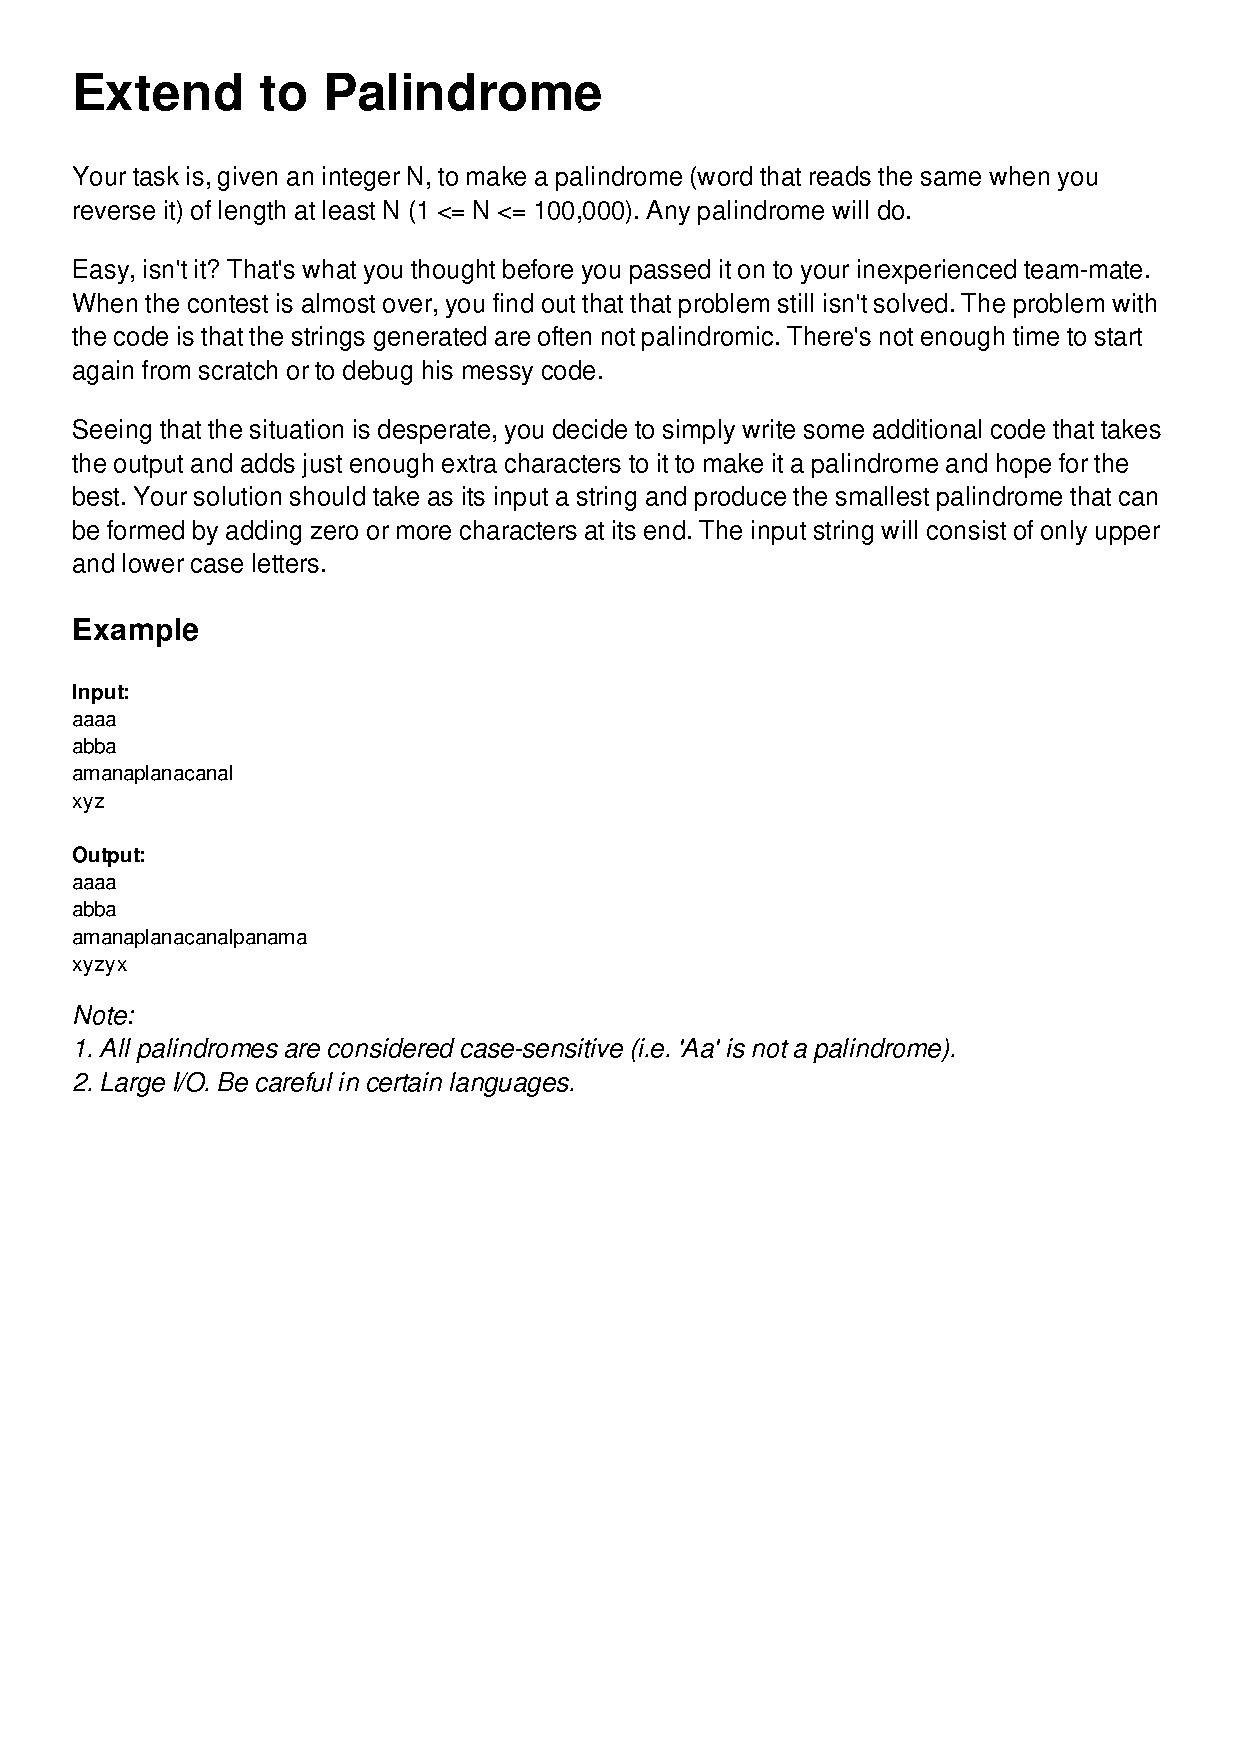
\includepdf[pages=-]{problemas/pdf/EPALIN.pdf}

\subsubsection{Implementación en C++}
\inputminted[linenos, frame=lines]{cpp}{problemas/cpp/EPALIN.cpp}

\begin{itemize}
\item En la línea \texttt{24} se hace una copia de la línea que se leyó
\item En la línea \texttt{26} se crea la cadena $r$.
\item En la línea \texttt{31, 32} se acompleta la cadena original para que sea un palíndromo.
\end{itemize}

\subsubsection{Implementación en Haskell}
\inputminted[linenos, frame=lines]{haskell}{problemas/haskell/EPALIN.hs}

\begin{itemize}
\item Al igual que el primer problema, se tratará la entrada y salida orientada a líneas con
la función \hsCode{interact} donde la función \hsCode{process} es la que hará \textit{el algorítmo}.
\item En la línea \texttt{8} se saca la reversa de la cadena de entrada, en la línea \texttt{9}
se crea la cadena $r$, en la línea \texttt{10} se crea la función de error. Finalmente en la línea
\texttt{13} con la \hsCode{drop :: Int -> [a] -> [a]} que regresa el sufijo de una lista
\texttt{xs} después de los primeros $n$ elementos, se obtiene la cadena faltante para completar el
palíndromo y en la línea \texttt{14} se concatena \texttt{xs} la cadena anterior.
\end{itemize}

\subsubsection{Resultado del juez}
\begin{figure}[H]
\centering
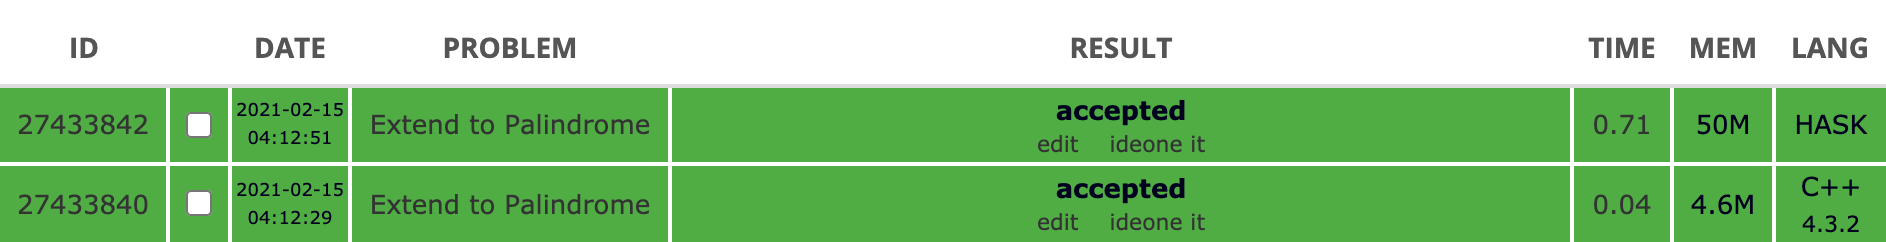
\includegraphics[width=\textwidth]{spoj/EPALIN-accepted-cpp-haskell}
\caption{El código fue aceptado por el juez en Haskell y C++}
\end{figure}

\newpage


\subsection{Encontrar todas las ocurrencias de un patrón en un texto}

\subsubsection{Análisis}
De los problemas anteriores este es quizás es el uso más \textit{canónico} del algoritmo
Knuth-Morris-Pratt per se, ya que solo se pide encontrar todas las posiciones 0-indexadas de
un patrón en un texto. Lo inlcuí porque ``la trampa'' de este problema es que mucha gente lo
resuelve con el algoritmo \textit{naïve} y simplemente el juez no lo aceptará. La complejidad como
ya se había comentado enteriormente, es $\Theta(m)$ en tiempo el preprocesamiento del patrón y
$\Theta(n)$ en encontrar las ocurrencias, en espacio toma complejidad $O(m)$.
%TODO: poner que está chido porque se pueden encontrar patrones que se overlapean

\subsubsection{Entrada}
Al igual que el primer problemas se leerá hasta EOF, y cada caso prueba consistirá de 3 líneas;
la primera será la longitud del patrón, seguida del patrón y después el texo.

\subsubsection{Salida}
Si hubo una(s) aparición(es) cada una será impresa en pantalla línea por línea. Si no, solamente
se imprirá un salto de línea.

\subsubsection{Ejemplos}
\begin{itemize}
\item El patón es \texttt{na} y el texto es \texttt{banananobano}, y hubo 2 apariciones del patrón
en las posiciones 2 y 4.
\begin{table}[h]
\centering
\begin{tabular}{|c|c|
>{\columncolor[HTML]{F5B7B1}}c|
>{\columncolor[HTML]{F5B7B1}}c|
>{\columncolor[HTML]{D7BDE2}}c|
>{\columncolor[HTML]{D7BDE2}}c|c|c|c|c|c|c|}
\hline
\texttt{b} & \texttt{a} & \texttt{n} & \texttt{a} & \texttt{n} & \texttt{a} & \texttt{n} &
\texttt{o} & \texttt{b} & \texttt{a} & \texttt{n} & \texttt{o} \\ \hline
\end{tabular}
\end{table}

\item El patón es \texttt{foobar} y el texto es \texttt{foo}, y no hubo ninguna aparición del
patrón.
\begin{table}[H]
\centering
\begin{tabular}{|c|c|c|}
\hline
\texttt{f} & \texttt{o} & \texttt{o} \\ \hline
\end{tabular}
\end{table}

\item El patón es \texttt{foobarfoo} y el texto es \texttt{barfoobarfoobarfoobarfoobarfoo}, y
hubo 4 apariciones del patrónen la posiciones 3, 9, 15 y 21.
\begin{table}[H]
\centering
\hspace*{-3cm}
\footnotesize
\begin{tabular}{|c|c|c|
>{\columncolor[HTML]{AED6F1}}c|
>{\columncolor[HTML]{AED6F1}}c|
>{\columncolor[HTML]{AED6F1}}c|
>{\columncolor[HTML]{AED6F1}}c|
>{\columncolor[HTML]{AED6F1}}c|
>{\columncolor[HTML]{AED6F1}}c|
>{\columncolor[HTML]{AED6F1}}c|
>{\columncolor[HTML]{AED6F1}}c|
>{\columncolor[HTML]{AED6F1}}c|c|c|c|c|c|c|c|c|c|c|c|c|c|c|c|c|c|c|c|}
\hline
\texttt{b} & \texttt{a} & \texttt{r} & \texttt{f} & \texttt{o} & \texttt{o} & \texttt{b} &
\texttt{a} & \texttt{r} & \texttt{f} & \texttt{o} & \texttt{o} & \texttt{b} & \texttt{a} &
\texttt{r} & \texttt{f} & \texttt{o} & \texttt{o} & \texttt{b} & \texttt{a} & \texttt{r} &
\texttt{f} & \texttt{o} & \texttt{o} & \texttt{b} & \texttt{a} & \texttt{r} & \texttt{f} &
\texttt{o} & \texttt{o} \\ \hline
\end{tabular}
\end{table}

\begin{table}[H]
\centering
\hspace*{-3cm}
\footnotesize
\begin{tabular}{|c|c|c|c|c|c|c|c|c|
>{\columncolor[HTML]{ABEBC6}}c|
>{\columncolor[HTML]{ABEBC6}}c|
>{\columncolor[HTML]{ABEBC6}}c|
>{\columncolor[HTML]{ABEBC6}}c|
>{\columncolor[HTML]{ABEBC6}}c|
>{\columncolor[HTML]{ABEBC6}}c|
>{\columncolor[HTML]{ABEBC6}}c|
>{\columncolor[HTML]{ABEBC6}}c|
>{\columncolor[HTML]{ABEBC6}}c|c|c|c|c|c|c|c|c|c|c|c|c|c|}
\hline
\texttt{b} & \texttt{a} & \texttt{r} & \texttt{f} & \texttt{o} & \texttt{o} & \texttt{b} &
\texttt{a} & \texttt{r} & \texttt{f} & \texttt{o} & \texttt{o} & \texttt{b} & \texttt{a} &
\texttt{r} & \texttt{f} & \texttt{o} & \texttt{o} & \texttt{b} & \texttt{a} & \texttt{r} &
\texttt{f} & \texttt{o} & \texttt{o} & \texttt{b} & \texttt{a} & \texttt{r} & \texttt{f} &
\texttt{o} & \texttt{o} \\ \hline
\end{tabular}
\end{table}

\begin{table}[H]
\centering
\hspace*{-3cm}
\footnotesize
\begin{tabular}{|c|c|c|c|c|c|c|c|c|c|c|c|c|c|c|
>{\columncolor[HTML]{F9E79F}}c|
>{\columncolor[HTML]{F9E79F}}c|
>{\columncolor[HTML]{F9E79F}}c|
>{\columncolor[HTML]{F9E79F}}c|
>{\columncolor[HTML]{F9E79F}}c|
>{\columncolor[HTML]{F9E79F}}c|
>{\columncolor[HTML]{F9E79F}}c|
>{\columncolor[HTML]{F9E79F}}c|
>{\columncolor[HTML]{F9E79F}}c|c|c|c|c|c|c|c|}
\hline
\texttt{b} & \texttt{a} & \texttt{r} & \texttt{f} & \texttt{o} & \texttt{o} & \texttt{b} &
\texttt{a} & \texttt{r} & \texttt{f} & \texttt{o} & \texttt{o} & \texttt{b} & \texttt{a} &
\texttt{r} & \texttt{f} & \texttt{o} & \texttt{o} & \texttt{b} & \texttt{a} & \texttt{r} &
\texttt{f} & \texttt{o} & \texttt{o} & \texttt{b} & \texttt{a} & \texttt{r} & \texttt{f} &
\texttt{o} & \texttt{o} \\ \hline
\end{tabular}
\end{table}

\begin{table}[H]
\centering
\hspace*{-3cm}
\footnotesize
\begin{tabular}{|c|c|c|c|c|c|c|c|c|c|c|c|c|c|c|c|c|c|c|c|c|
>{\columncolor[HTML]{EDBB99}}c|
>{\columncolor[HTML]{EDBB99}}c|
>{\columncolor[HTML]{EDBB99}}c|
>{\columncolor[HTML]{EDBB99}}c|
>{\columncolor[HTML]{EDBB99}}c|
>{\columncolor[HTML]{EDBB99}}c|
>{\columncolor[HTML]{EDBB99}}c|
>{\columncolor[HTML]{EDBB99}}c|
>{\columncolor[HTML]{EDBB99}}c|c|}
\hline
\texttt{b} & \texttt{a} & \texttt{r} & \texttt{f} & \texttt{o} & \texttt{o} & \texttt{b} &
\texttt{a} & \texttt{r} & \texttt{f} & \texttt{o} & \texttt{o} & \texttt{b} & \texttt{a} &
\texttt{r} & \texttt{f} & \texttt{o} & \texttt{o} & \texttt{b} & \texttt{a} & \texttt{r} &
\texttt{f} & \texttt{o} & \texttt{o} & \texttt{b} & \texttt{a} & \texttt{r} & \texttt{f} &
\texttt{o} & \texttt{o} \\ \hline
\end{tabular}
\end{table}

\end{itemize}

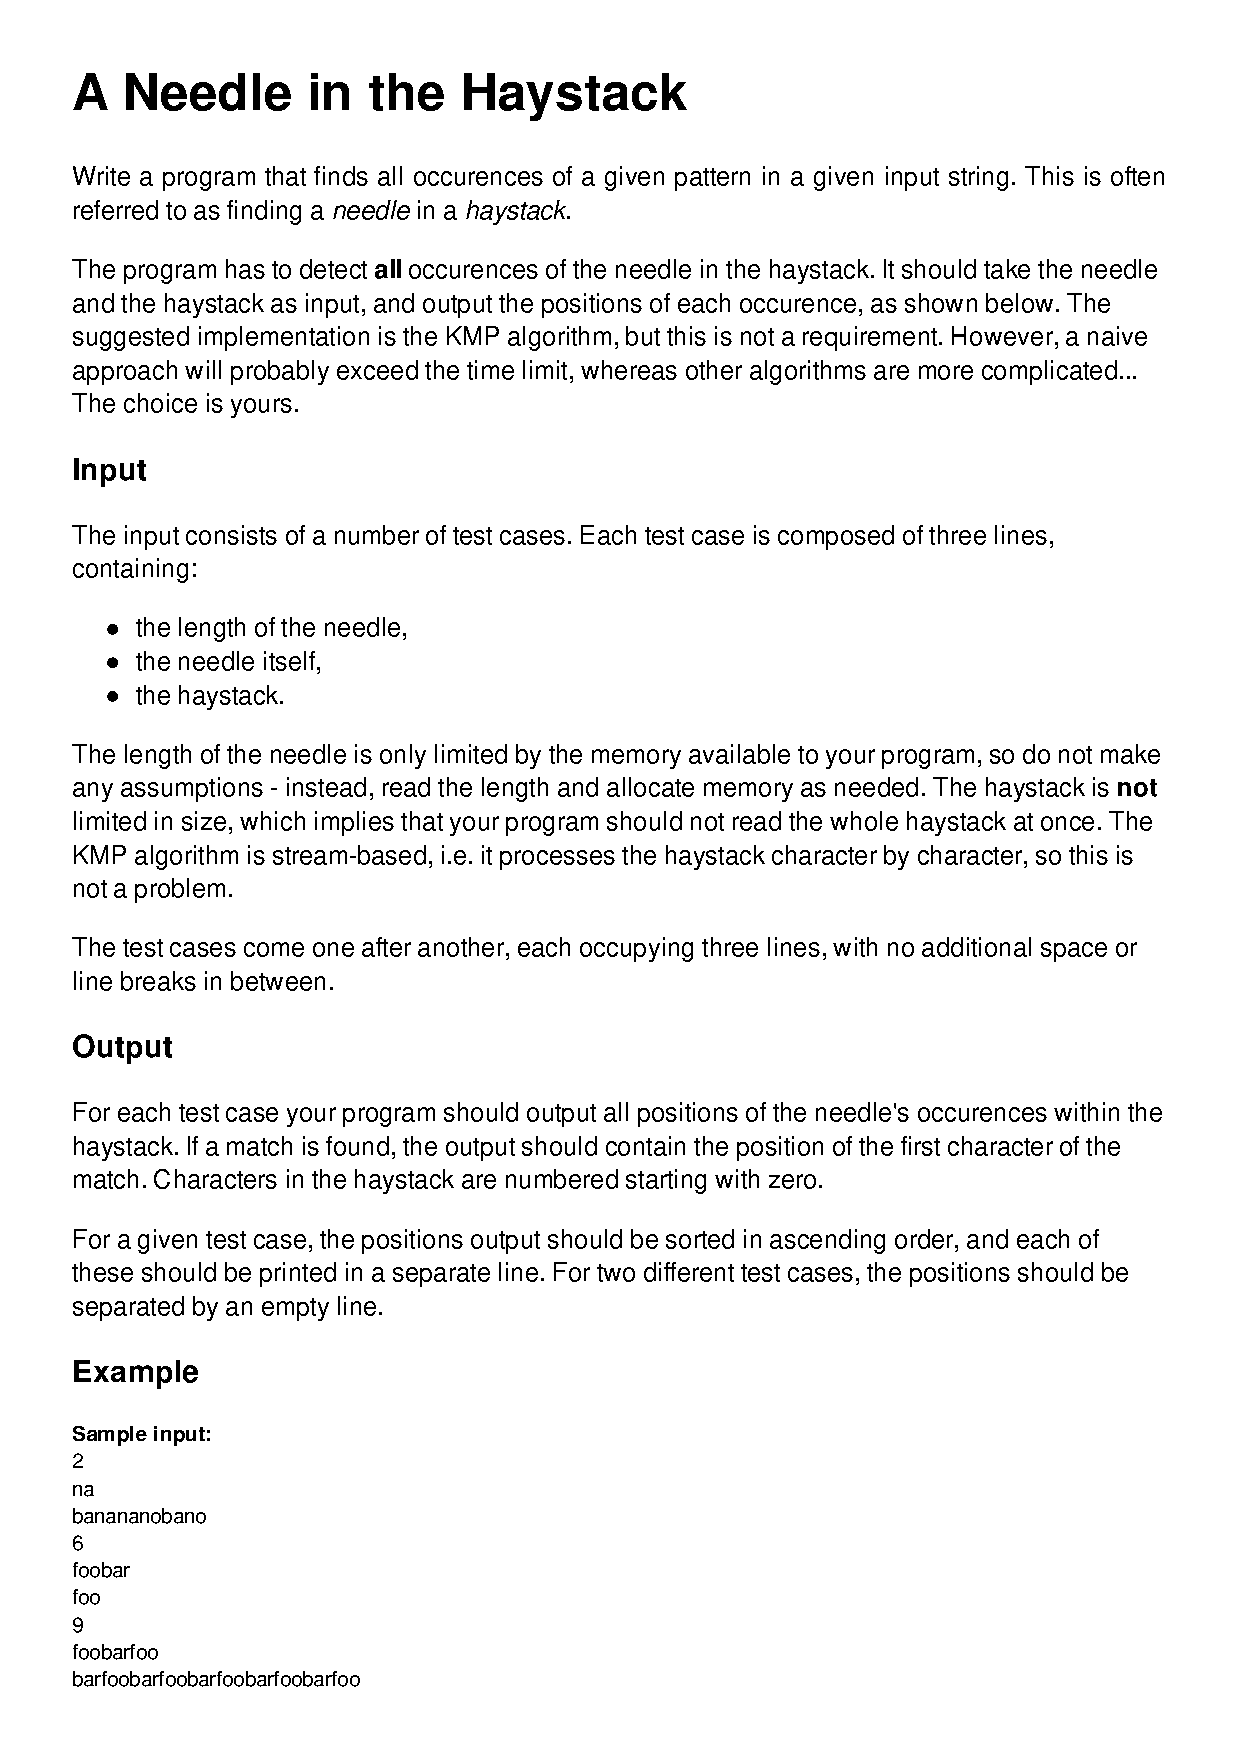
\includepdf[pages=-]{problemas/pdf/NHAY.pdf}

\subsubsection{Implementación en C++}
\inputminted[linenos, frame=lines, fontsize=\footnotesize]{cpp}{problemas/cpp/NHAY.cpp}

\subsubsection{Implementación en Haskell}
\inputminted[linenos, frame=lines]{haskell}{problemas/haskell/NHAY.hs}

\begin{itemize}
\item Al ser un programa orientado a líneas, solo se prestará atención a la función
\hsCode{process} y \hsCode{parse}.

En la función \hsCode{parse} se usa para \textit{procesar} de tres en tres líneas y cada caso
prueba verlo como una sola tupla. En la función \hsCode{process} en la línea \texttt{12} busca
las apariciones del patrón en el texto, seguido en la línea \texttt{14} verifica si es una lista
vacía, si lo es solamente regresa un salto de línea, si no con la función
\hsCode{intercalate :: [a] -> [[a]] -> [a]} que inserta el primer argumento entre cada elemento
de la lista y concatena el resultado, pone un salto de línea entre cada índice de cada ocurrencia.
\end{itemize}

\subsubsection{Resultado del juez}
\begin{figure}[h]
\centering
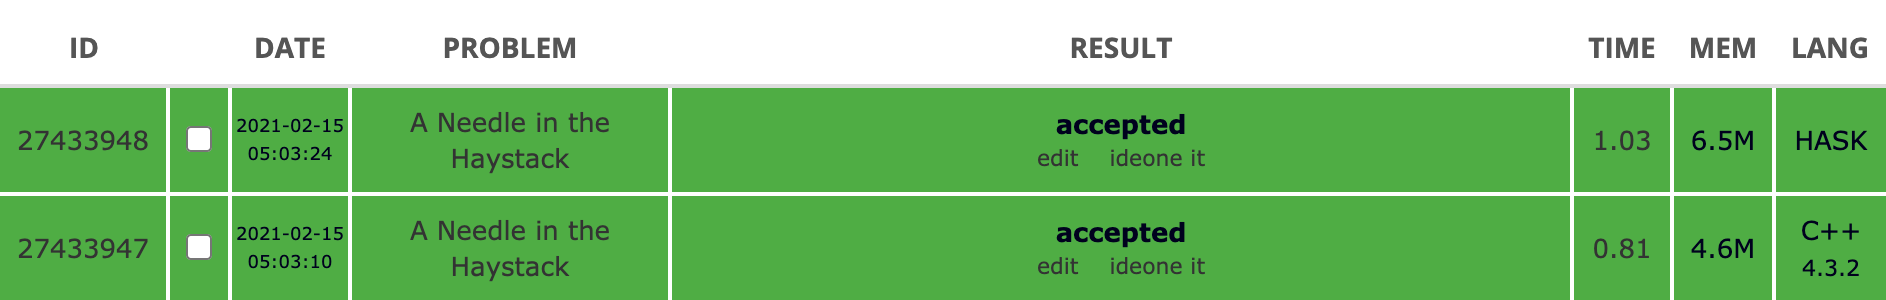
\includegraphics[width=\textwidth]{spoj/NHAY-accepted-cpp-haskell}
\caption{El código fue aceptado por el juez en Haskell y C++}
\end{figure}

% TODO: poner que puedo optimizar la entrada con Data.ByteString.Char8